\documentclass{article}
\usepackage{graphicx}
\usepackage{float}
\usepackage{caption}
\usepackage{subcaption}
\usepackage{gensymb}
\usepackage[utf8]{inputenc}
\usepackage[a4paper, total={6in, 8in}]{geometry}

\renewcommand{\thesubsection}{\thesection.\alph{subsection}}

\begin{document}

\author{Antonella Dellanzo - Daiana Delgadino}
\title{Guía 4: DFT con Matlab}
\date{}
\maketitle

\section*{Ejercicio 1}

\subsection*{Ejercicio a}

El método para este ejercicio se llama \textbf{ej1a} y toma como parámetro un número entero \textit{N} que indica la dimensión en la cual se desea obtener la base de Fourier en 1-D. Se generan dos figuras:
\begin{itemize}
\item La primera muestra la parte real de la base de Fourier en 1-D para cada valor de $N$.
\item La segunda muestra la parte imaginaria de la base de Fourier en 1-D para cada valor de $N$.
\end{itemize}
Por ejemplo, para $N=8$ como pedía el enunciado, se obtiene lo siguiente:

\begin{figure}[H]
    \begin{subfigure}{0.5\textwidth}
        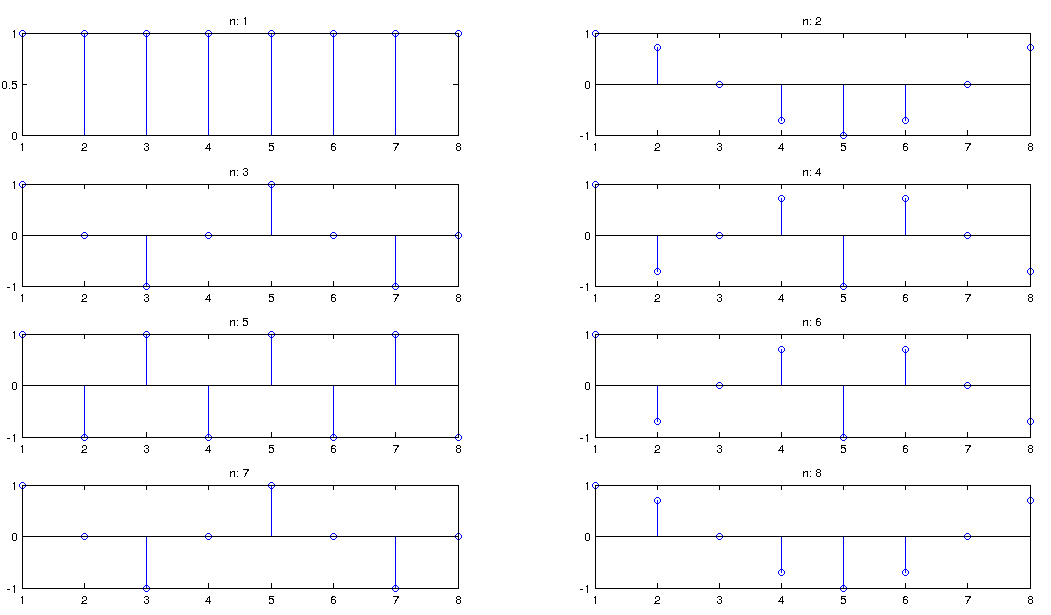
\includegraphics[width=0.9\textwidth]{parteReal8.png}
    \subcaption{Parte Real con $N=8$}
    \end{subfigure}\hfill
    \begin{subfigure}{0.5\textwidth}
        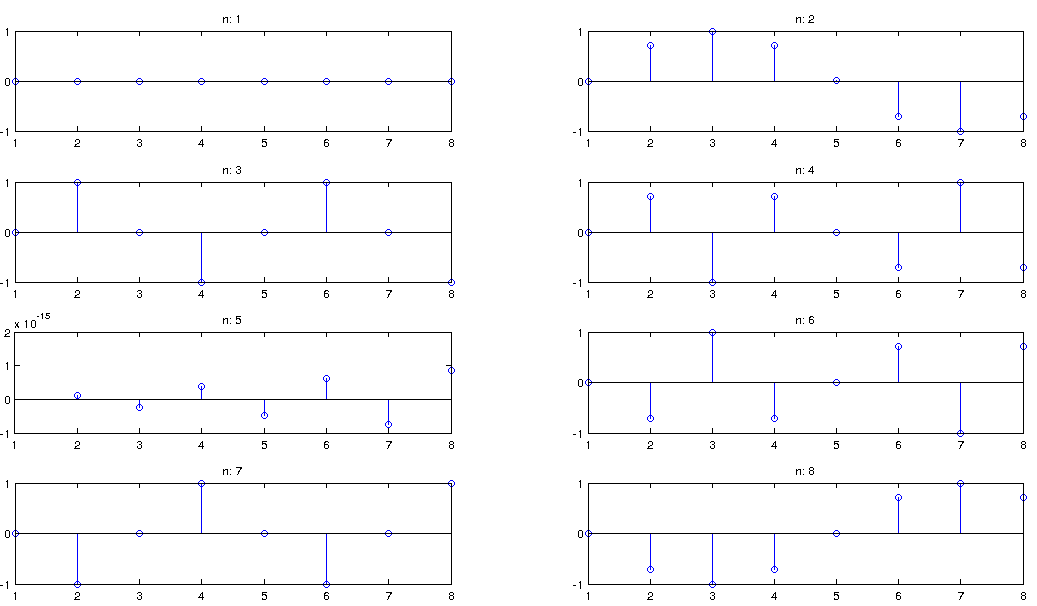
\includegraphics[width=0.9\textwidth]{parteImagN8.png}
    \subcaption{Parte Imaginaria con $N=8$}
    \end{subfigure}
    \caption{Bases de Fourier en 1-D}
\end{figure}

\subsection*{Ejercicio b}

El método para este ejercicio se llama \textbf{ej1b} y toma como parámetro de entrada dos números enteros \textit{N} y \textit{M} que indican las dimensiones en las que se busca obtener la base de Fourier en 2-D. Se generan dos figuras:
\begin{itemize}
\item La primera muestra la parte real de la base de Fourier en 2-D para cada valor de $N$ y $M$.
\item La segunda muestra la parte imaginaria de la base de Fourier en 2-D para cada valor de $N$ y $M$.
\end{itemize} Por ejemplo, para $N=8, M=8$ como pedía el enunciado, se obtiene lo siguiente:

\begin{figure}[H]
        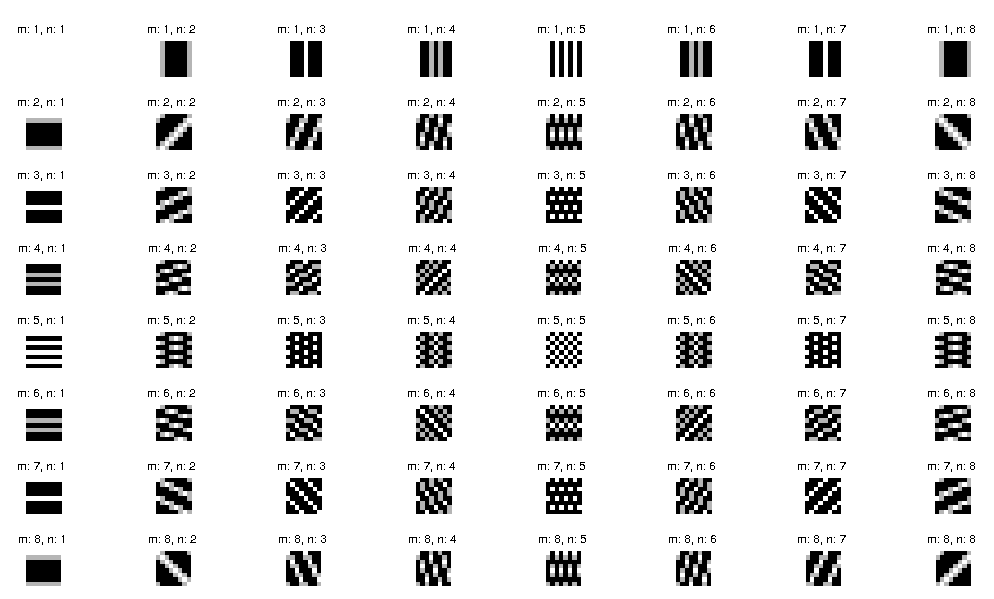
\includegraphics[width=0.9\textwidth]{ej1bRealN8M8.png}
    \caption{Parte Real $N=8,M=8$ de la base de Fourier en 2-D}
\end{figure}
\begin{figure}[H]
        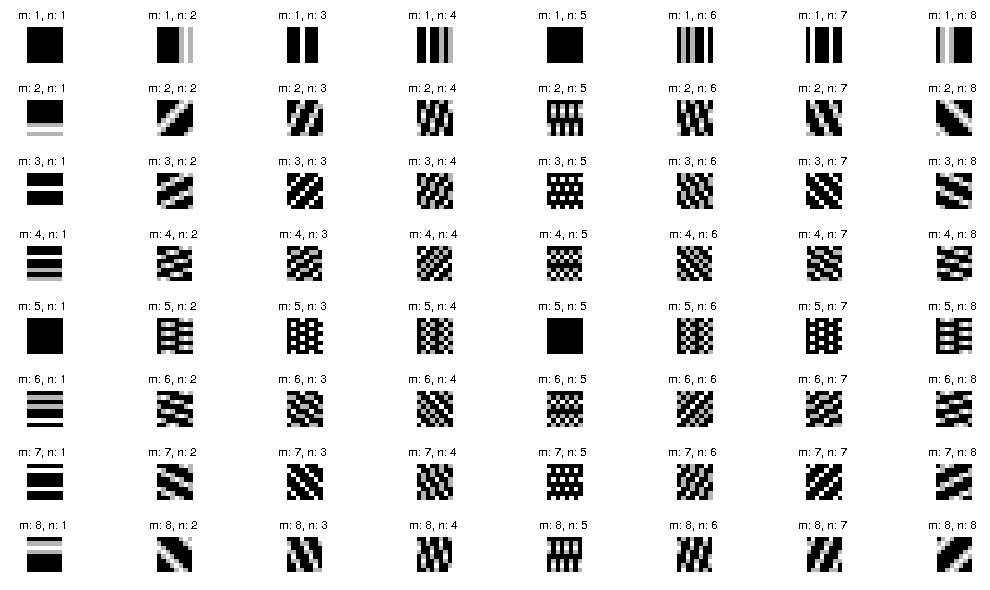
\includegraphics[width=0.9\textwidth]{ej1bImagN8M8.png}
    \caption{Parte Imaginaria $N=8,M=8$ de la base de Fourier en 2-D}
\end{figure}

\section*{Ejercicio 2}
El método para este ejercicio se llama \textbf{ej2} y no toma parámetros de entrada. Como resultado genera una figura mostrando el vector original (en este caso utilizamos el vector $[ 1,1,1,1,1,1,1,1,1,0,0,0,0,0,0,0 ]$), el valor absoluto de Fourier aplicado al vector y tres vectores resultantes:
\begin{itemize}
\item \textit{Vector sin frecuencias bajas:} Resultante de quitarle aquellos valores tal que $abs(fft(vector)) < 0.2$.
\item \textit{Vector sin frecuencias altas:} Resultante de quitarle aquellos valores tal que $abs(fft(vector)) > 1.0$.
\item \textit{Vector sin frecuencias intermedias:} Resultante de quitarle aquellos valores tal que $0.2 < abs(fft(vector)) < 1.0$.
\end{itemize}

Los valores para remover los determinamos luego de obtener el valor absoluto de la transformada de fourier del vector. Para calcular la transformada de Fourier y la antitransformada, nos generamos dos métodos: \textbf{DFT} y \textbf{IDFT}. Estos toman como parámetro de entrada un vector al cual se le aplica la transformada y antitransformada correspondientemente. 

Para el vector del enunciado, se obtuvo el siguiente resultado:

 \begin{figure}[H]
    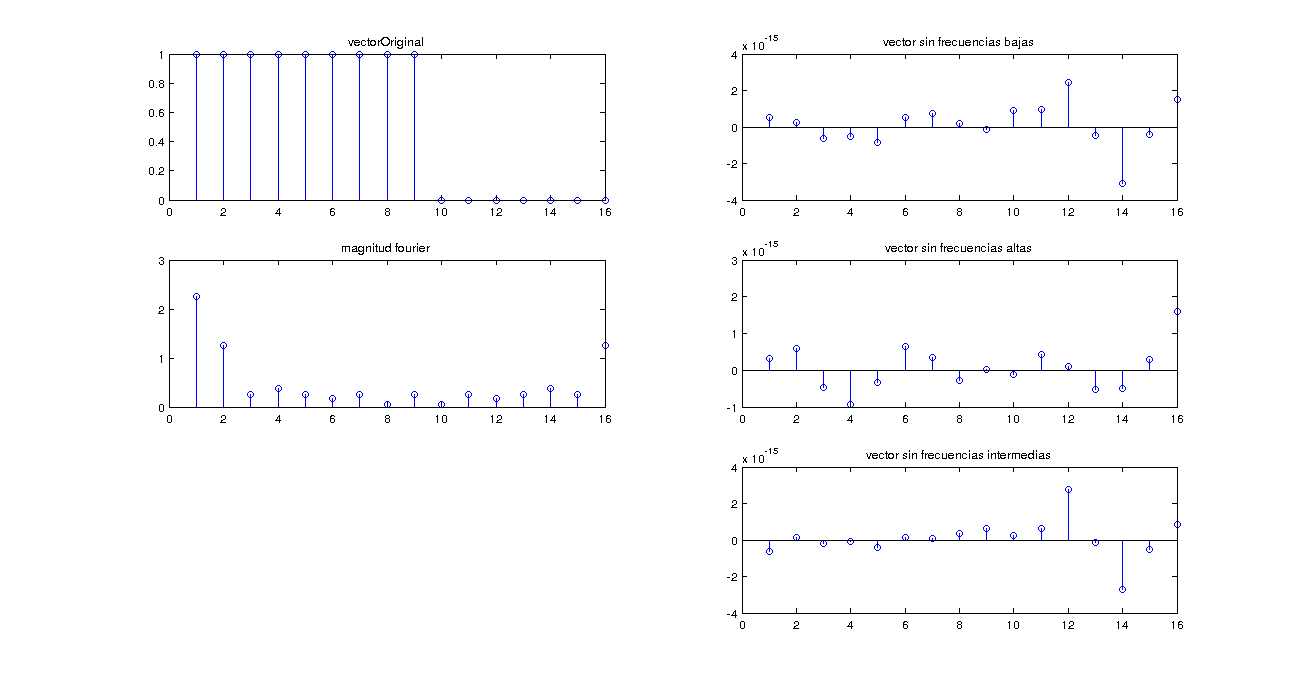
\includegraphics[width=0.9\textwidth]{ej2.png}
\end{figure}

\section*{Ejercicio 3}

El método para este ejercicio se llama \textbf{ej3} y no toma parámetros de entrada. Como resultado, genera las 10 figuras pedidas en el ejercicio, en las cuales se muestra: la imagen original, el valor absoluto de la transformada de Fourier de la imagen shifteada y la antitransformada de la imagen. Para cada figura, generamos un método que genera una imagen con lo pedido, los cuales son: \textit{cuadrado}, \textit{cuadradoTransladado}, \textit{rectangulo}, \textit{rectangulos}, \textit{lineaVertical}, \textit{lineaVerticalRotada45}, \textit{lineaVerticalRotada90}, \textit{lineasVerticales}, \textit{lineasVerticalesRotadas45} y \textit{lineasVerticalesRotadas90}. Para la transformada de Fourier en 2-D, generamos dos métodos: \textbf{DFT2D} y \textbf{IDFT2D}, que toman como parámetro de entrada una matriz y retornan la transformada y antitransformada de Fourier correspondientemente. Por ejemplo, para ciertas figuras, obtuvimos lo siguiente:

\begin{figure}[H]
    \begin{subfigure}{0.5\textwidth}
        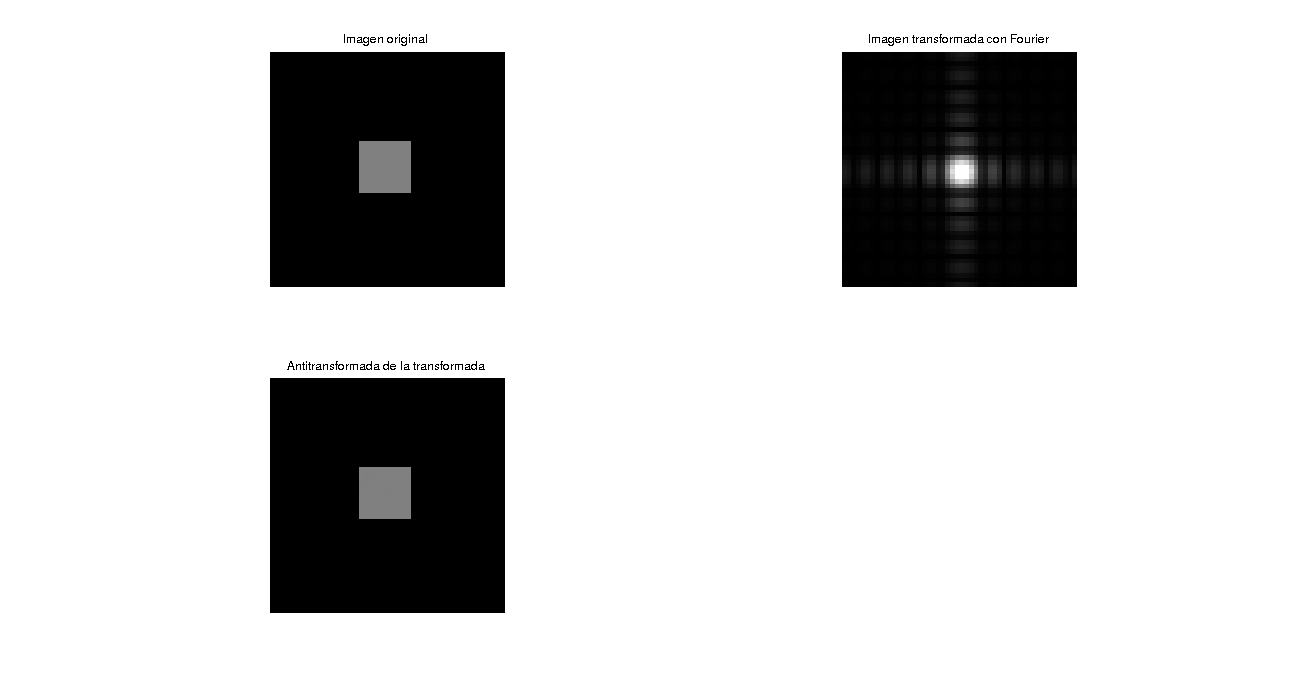
\includegraphics[width=0.9\textwidth]{ej3.png}
    \subcaption{Ejercicio 3 aplicado a un cuadrado}
    \end{subfigure}\hfill
    \begin{subfigure}{0.5\textwidth}
        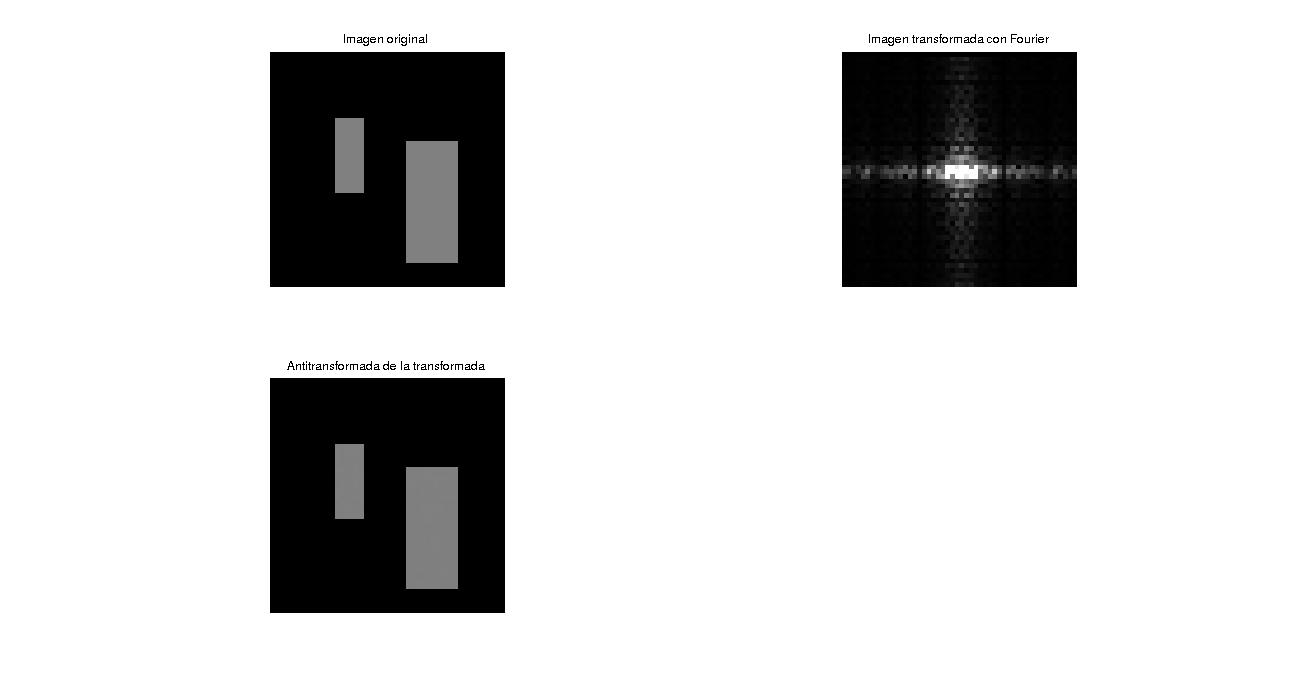
\includegraphics[width=0.9\textwidth]{ej3-otro.png}
    \subcaption{Ejercicio 3 aplicado a un dos rectángulos de distinto tamaño}
    \end{subfigure}\hfill
    \begin{subfigure}{0.5\textwidth}
        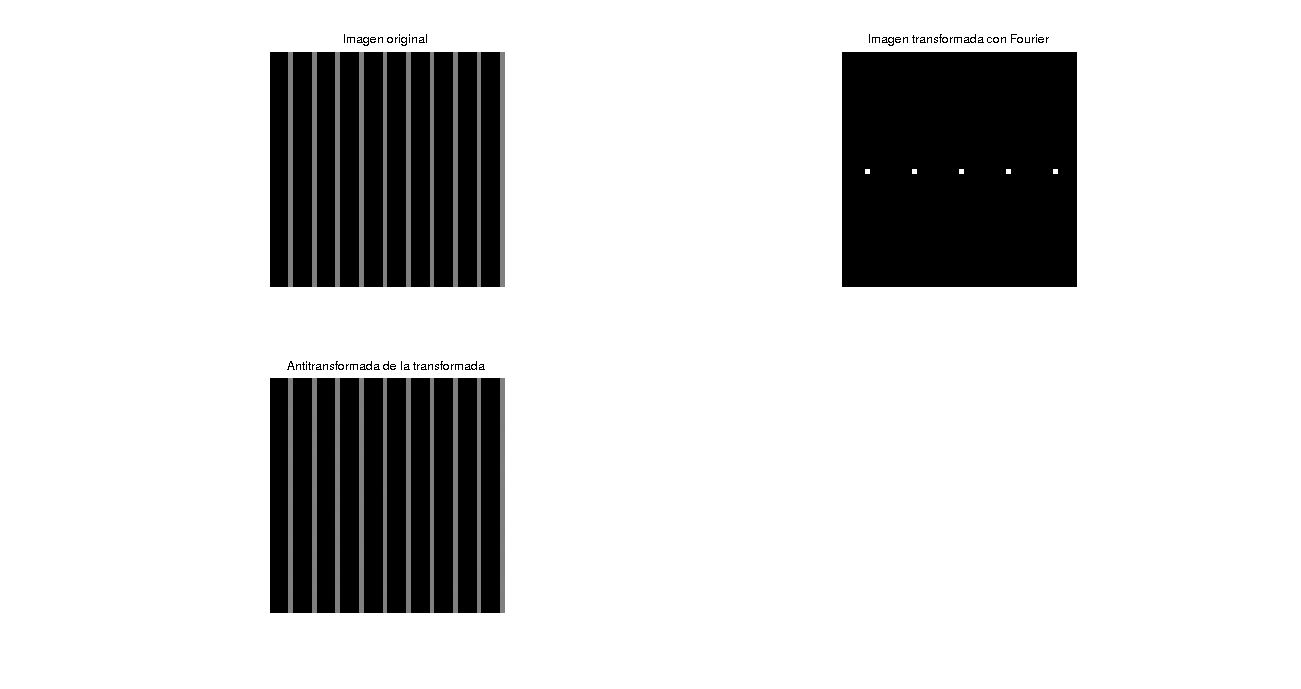
\includegraphics[width=0.9\textwidth]{ej3-otro2.png}
    \subcaption{Ejercicio 3 aplicado a lineas verticales}
    \end{subfigure}\hfill
    \begin{subfigure}{0.5\textwidth}
        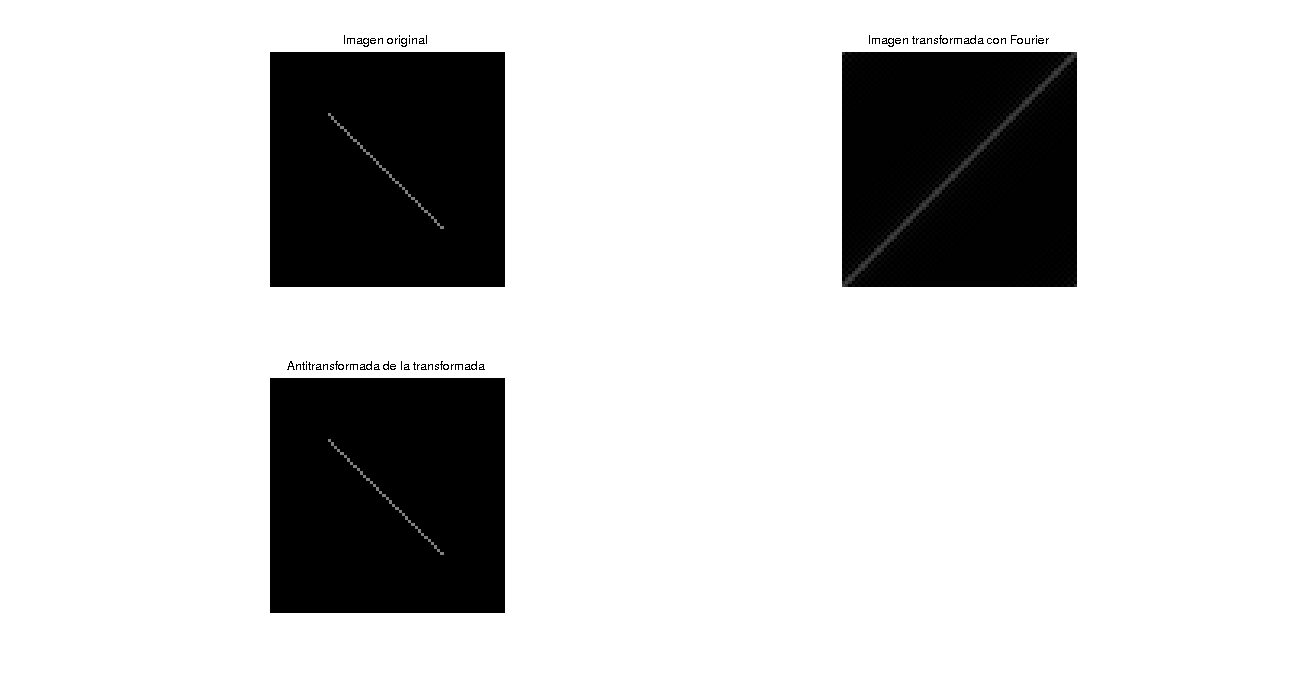
\includegraphics[width=0.9\textwidth]{ej3-otro3.png}
    \subcaption{Ejercicio 3 aplicado a una línea en diagonal}
    \end{subfigure}
\end{figure}

\section*{Ejercicio 4}

El método para este ejercicio se llama \textbf{ej4} y toma parámetros de entrada dos imágenes. Este método genera una figura que muestra cuatro imágenes: las dos imágenes originales, una imagen mostrando el resultado de componer el módulo de la primera y la fase de la segunda, y una tercera mostrando el resultado de la composición del módulo de la segunda con la fase de la primera. Por ejemplo, para la imagen de lena y el ladrillo, se obtuvo lo siguiente, en lo cual se puede observar que el aporte de la fase es mucho mayor a la del módulo:

\begin{figure}[H]
\centering
    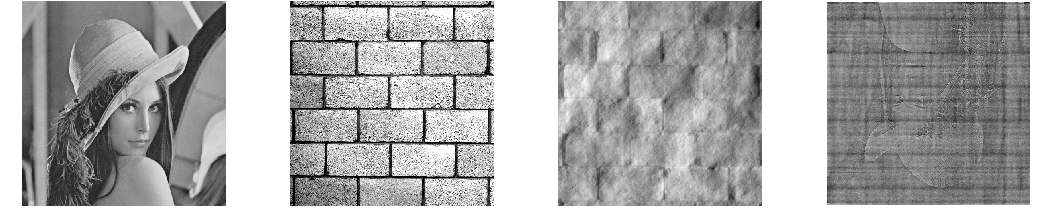
\includegraphics[width=1\textwidth]{ej4.png}
    \caption{Ejercicio 4 aplicado a la imagen de lena y ladrillos}
\end{figure}

\section*{Ejercicio 5}

El método para este ejercicio se llama \textbf{ej5} y no toma parámetros de entrada. Se generan dos figuras:
\begin{itemize}
\item La primera muestra la imagen de lena sumada a una imagen que posee varias líneas verticales blancas generadas con el método \textbf{lineas512x512} y otra imagen mostrando el logaritmo del valor absoluto de la transformada de fourier de esta imagen compuesta.
\item La segunda imagen muestra el resultado de quitar de la imagen las frecuencias que se encontraban en la fila 257 de la transformada de Fourier y luego aplicar la antitransformada para obtener la imagen resultante.
\end{itemize}

Estas son las imágenes obtenidas:

\begin{figure}[H]
        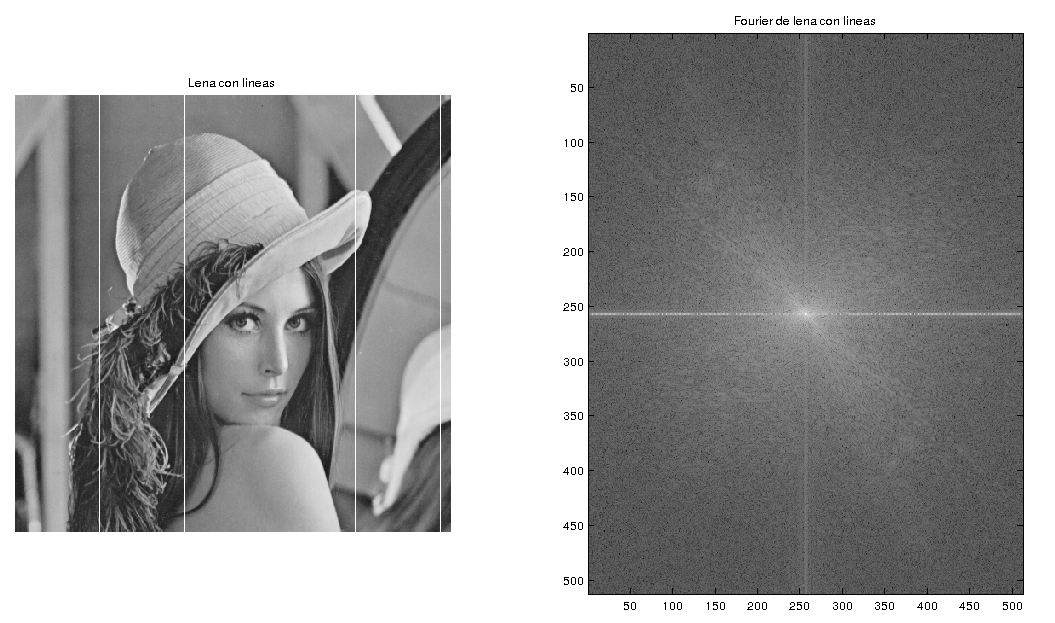
\includegraphics[width=0.9\textwidth]{ej5.png}
    \caption{Imagen de Lena con líneas y la transforamada de Fourier de la imagen}
\end{figure}
\begin{figure}[H]
\centering
    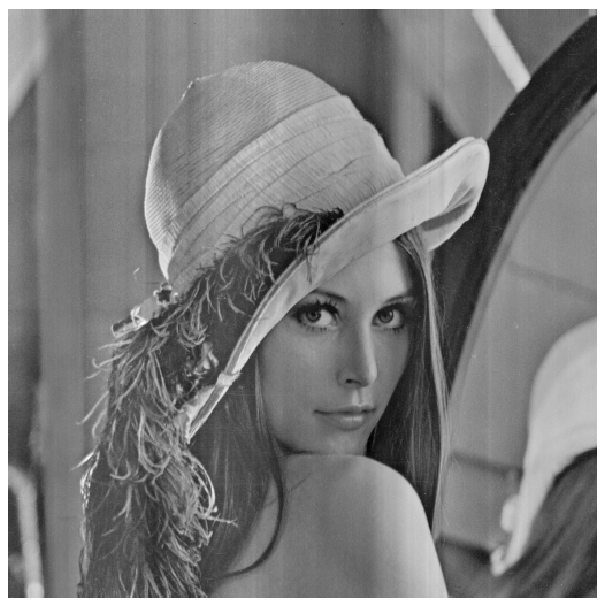
\includegraphics[width=0.5\textwidth]{lenaSinLineas.png}
    \caption{Imagen de Lena luego de remover las líneas}
\end{figure}

Para obtener la transformada y antitransformada de Fourier, utilizamos las funciones provistas por matlab \textit{fft2} e \textit{ifft2} debido a que las implementadas por nosotras demoraban mucho. Luego, realizamos un análisis sobre la transformada de Fourier para evaluar cuáles eran las frecuencias que debíamos remover para poder quitar las líneas de la imagen (obteniendo que éstas eran las que se encontraban en la fila 257). Luego, colocamos los valores de dicha fila en 0 y obtuvimos la antitransformada de Fourier para generar la imagen final.

\section*{Ejercicio 6}

El método para este ejercicio se llama \textbf{ej6} y toma como parámetro de entrada un número entero $N$ que indica la cantidad de muestras que se tomarán de las funciones $f$ y $g$. Estos valores se obtienen generando valores de tipo \textit{double} al azar entre 0 y 1 con el método \textit{rand} de matlab. En este ejercicio aplicamos fourier a la convolución de $f$ y $g$ por un lado, y por otro multiplicamos la transformada de Fourier punto a punto de $f$ y $g$ (ambas operaciones se realizan sobre los vectores de longitud $N$ generados que simulan muestras obtenidas de las funciones en $x$, con $1\leq x \leq N$). Generamos una figura mostrando la parte real e imaginaria de cada resultado. Por ejemplo, para $N=10$ se obtienen las siguientes figuras, en los que se puede observar que son equivalentes los resultados:

\begin{figure}[H]
    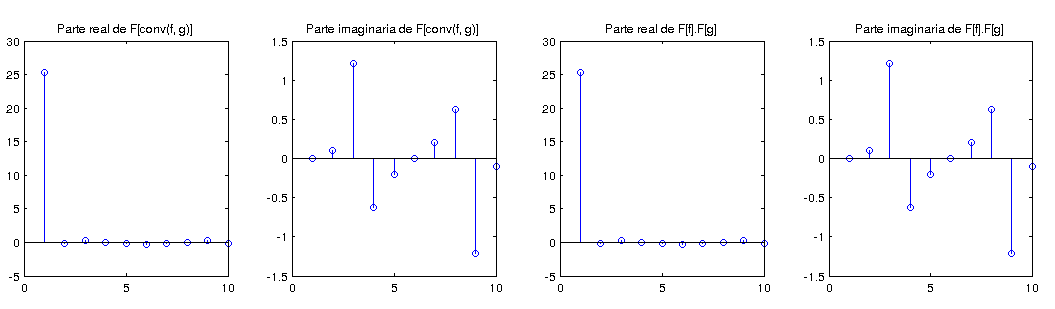
\includegraphics[width=1\textwidth]{ej6.png}
\end{figure}

\end{document}